\section{Model Room Illuminance Calculation}
The algorithm was tested on model room of dimension $\left(10 \times 5 \times 4\right)$~m. Any barriers or equipment were not considered. Pure diffuse reflections were considered with facets reflectance:
\begin{itemize}
	\item $\rho = 0.2$ for floor,
	\item $\rho = 0.5$ for walls,
	\item $\rho = 0.7$ for ceiling.
\end{itemize}
Each facet has the same dimension $\left(0.25 \times 0.25\right)$~m. $4$~reflections were evaluated for each solution. High count of reflection slows down the algorithm. It was found out that there was increase less than $10$~\% in resulting illuminance after the 4\textsuperscript{th} reflection. This fact was tested in simulation after only one lamp was presented in the middle of the rooms ceiling. The result is graphically shown in Figure~\ref{fig:reflDif}.

\begin{figure}[htb]
  \centering
  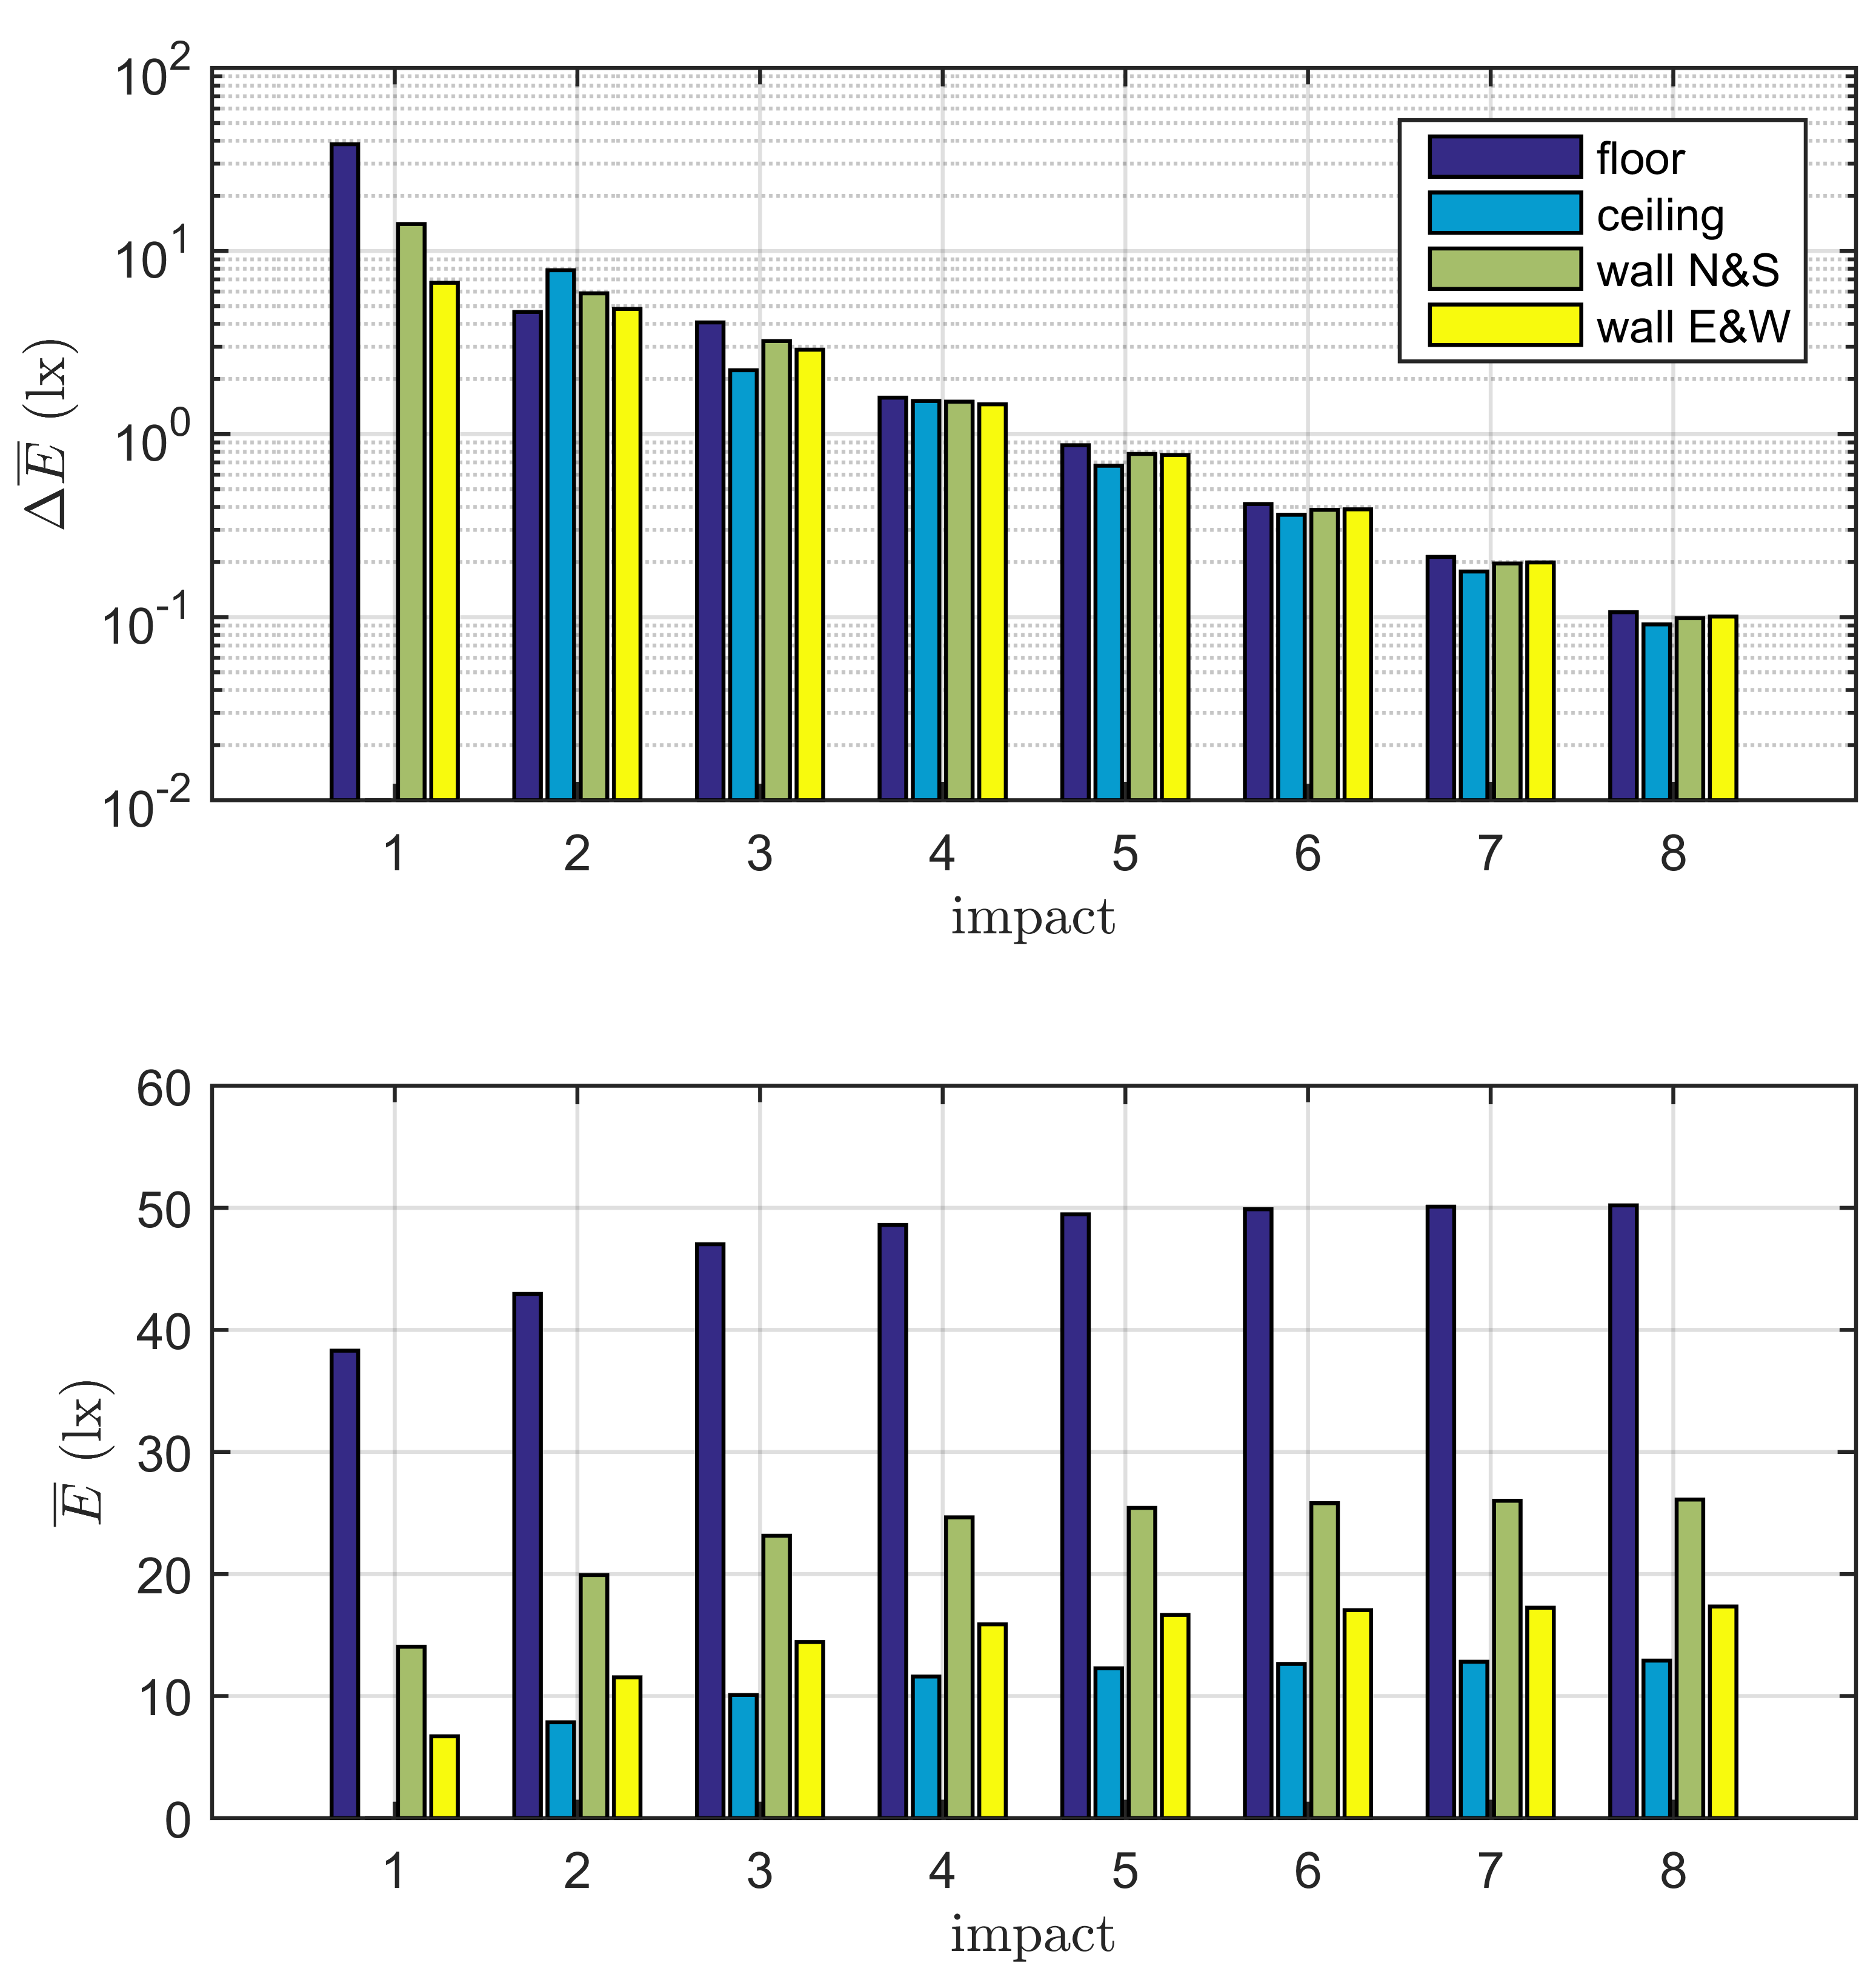
\includegraphics[width=\columnwidth]{reflDif}
  \caption{Increase of the wall average illuminance for one lamp in the room ceiling center according to the count of reflections.}
  \label{fig:reflDif}
\end{figure}

The grid of control points was uniformly placed on the reference plane with distances 25~cm. The luminaires were placed in rectangular area on the ceiling that starts $0.5$~m from the E\&W walls and $0.4$~m from N\&S walls. All further presented results were evaluated for the same luminaire  MSTR~SLB~4x18W. The elumdata were taken from the software "Building Design". All placed luminaires had the same orientation, which was described by normal vector of $C0^\circ-C180^\circ$ plane in each test. The luminuous intensity curve is shown in Figure~\ref{fig:IDiag}. The dimension of the luminaire were considered $595\times 595\times 80$~mm.

\begin{figure}[htb]
  \centering
  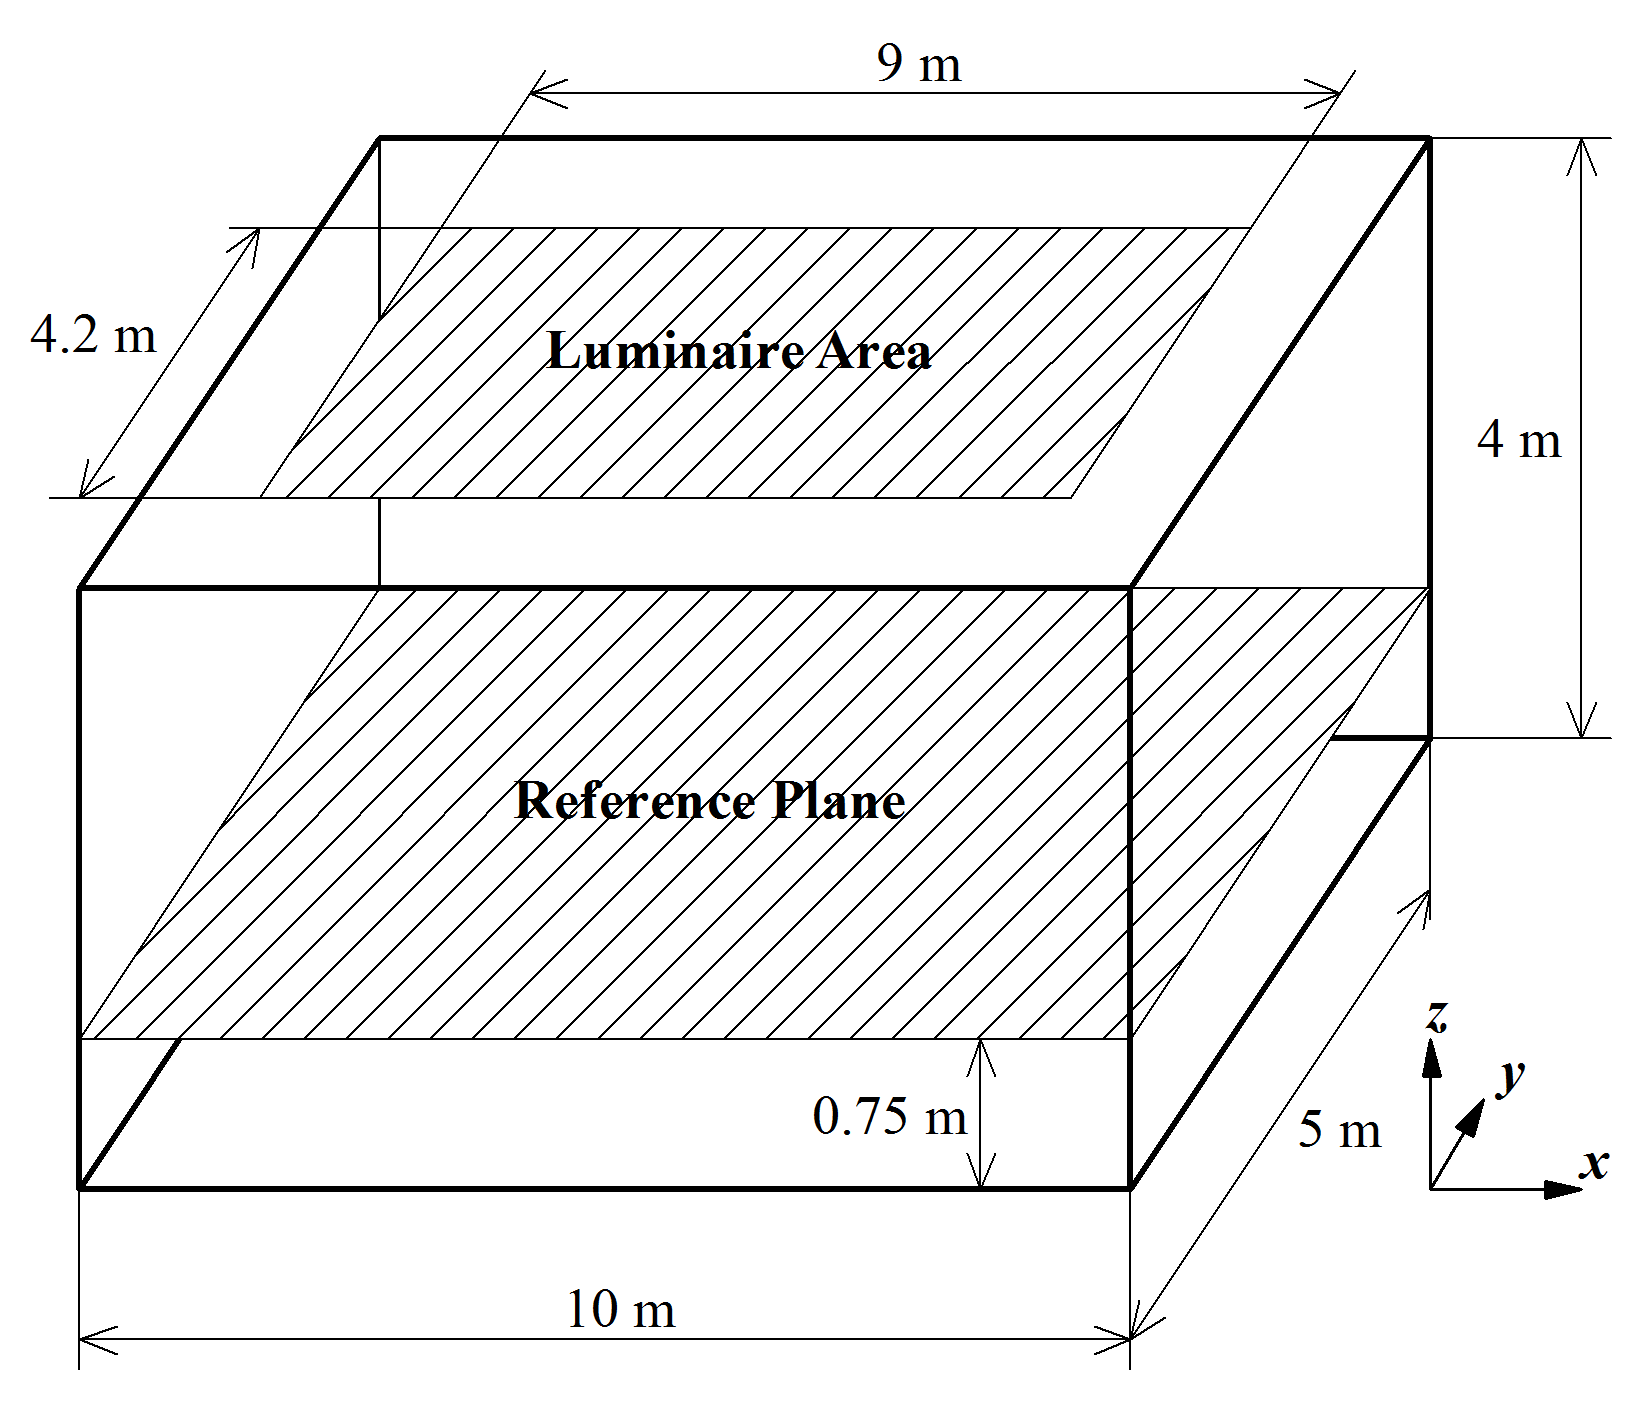
\includegraphics[width=\columnwidth]{modRoom}
  \caption{Model room dimensions}
  \label{fig:modRoom}
\end{figure}

\begin{figure}[htb]
  \centering
  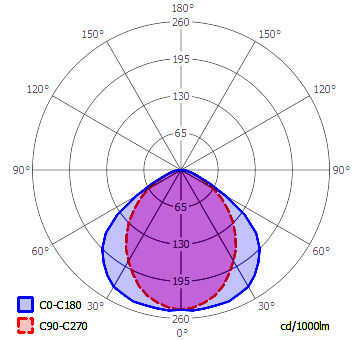
\includegraphics[width=0.8\columnwidth]{IDiag}
  \caption{Luminous intensity distribution curve of the luminaire sample}
  \label{fig:IDiag}
\end{figure}